% =========================================================================
% Supplementary Material -- HumanBrain Cross-Species CIS
% =========================================================================
% All values quoted from frozen artifacts; mirrors 10_REPORT/
% SUPPLEMENTARY_MATERIAL.md (S1-S14) and 08_FIGURES/FIGURE_CAPTIONS.md.
% =========================================================================
\documentclass[11pt,a4paper]{article}

\usepackage[T1]{fontenc}
\usepackage[utf8]{inputenc}
\usepackage{newtxtext,newtxmath}
\usepackage[margin=2.4cm]{geometry}
\usepackage{graphicx}
\usepackage{booktabs}
\usepackage{url}
\usepackage{amsmath} % amssymb omitted: newtxmath provides AMS symbols
\usepackage{microtype}
\usepackage{xcolor}
\usepackage[font=small,labelfont=bf]{caption}
\usepackage{titlesec}
\usepackage[hidelinks,colorlinks=true,linkcolor=blue!50!black,citecolor=blue!50!black,urlcolor=blue!50!black]{hyperref}

\graphicspath{{figures/}}

\renewcommand{\thefigure}{S\arabic{figure}}
\renewcommand{\thetable}{S\arabic{table}}
\renewcommand{\thesection}{S\arabic{section}}
\newcommand{\CIS}{\mathrm{CIS}}

\title{\bfseries Supplementary Material for\\
``Control-impact architecture of the human structural connectome: degree
dominance, a small near-universal residual, and a cross-scale architectural
comparison with the fly connectome''}
\author{Harsha Vardhan Malipeddi\\[2pt]\small Independent Researcher}
\date{}

\begin{document}
\maketitle

\section{Dataset provenance}
Zenodo~19796783 (AOMIC-ID1000 structural connectomes), CC-BY-4.0; 10 zips,
7{,}067{,}175{,}601 bytes, byte-exact vs.\ API; CRC clean; 900 subjects
$\times$ 7 atlases $\times$ 4 variants. Verification:
\texttt{../00\_Metadata/AOMIC\_VERIFICATION\_REPORT.md}; checksums:
\texttt{../00\_Metadata/CHECKSUMS\_AOMIC.sha256}. Raw zips are read-forever
(never modified).

\section{QC rules}
Pre-registered property-based QC (E02, CIS-blind): dimension mismatch, NaN,
Inf, asymmetry $>10^{-9}$, negative off-diagonals, isolated nodes, strength
IQR, density IQR, multi-component ($>1$ non-trivial component). Cohort:
801/900 pass; 94 isolated-node + 5 strength-IQR flags; flagged subjects
retained, never deleted. Population QC summary: Table~\ref{tab:sqc};
flag distributions: Fig.~\ref{fig:suppqc}. Artifacts:
\texttt{03\_BASELINE/qc\_primary.csv}, \texttt{BASELINE\_RESULTS.md},
\texttt{01\_RAW\_PROBES/raw\_qc\_report.csv}.

% Auto-generated float (caption + label inside the file):
% AUTO-GENERATED from 09_TABLES/table_03_qc_summary.csv -- do not edit numbers by hand.
\begin{table}[!t]
\centering\small
\caption{Population QC summary over the 801-subject primary cohort (frozen
\texttt{table\_03\_qc\_summary.csv}; mean and median across subjects, primary
configuration). Strength is in SIFT-weighted streamline-count units.}
\label{tab:sqc}
\begin{tabular}{lrr}
\toprule
Metric & Mean & Median \\
\midrule
Nodes per graph & 456.0 & 456.0 \\
Raw density & 0.4515 & 0.4623 \\
Isolated nodes after threshold (mean) & 0.1200 & 0.0000 \\
Multi-node components (mean) & 1.0000 & 1.0000 \\
Giant-component fraction & 0.9997 & 1.0000 \\
Global efficiency $E_0$ & 0.5467 & 0.5468 \\
Mean node strength & 15,588.4 & 15,527.4 \\
flag\_density\_iqr & 0.0000 & 0.0000 \\
flag\_strength\_iqr & 0.0056 & 0.0000 \\
flag\_components & 0.0000 & 0.0000 \\
flag\_isolated & 0.1044 & 0.0000 \\
n\_qc\_pass & 801.0 & 801.0 \\
\bottomrule
\end{tabular}
\end{table}


\begin{figure}[!t]
\centering
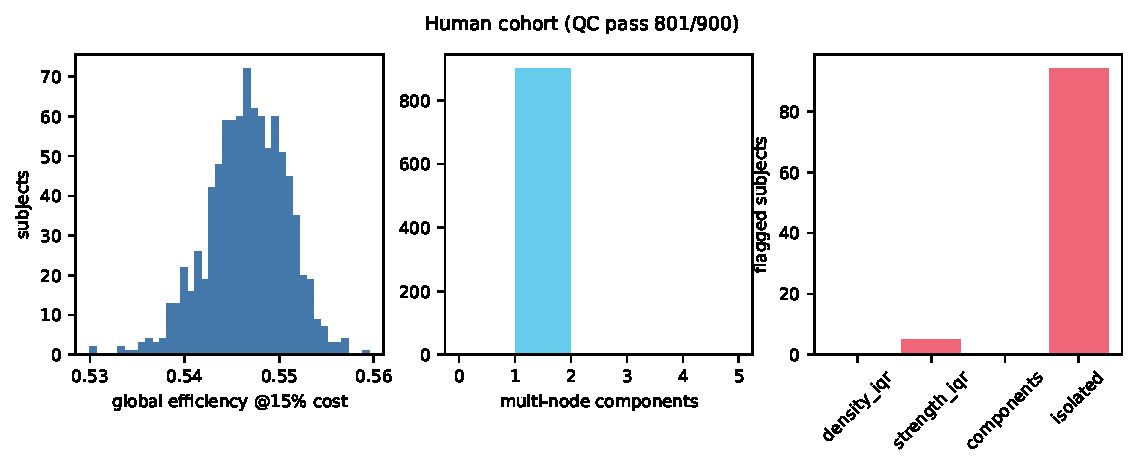
\includegraphics[width=\textwidth]{fig02_population_qc.pdf}
\caption{\textbf{Population QC (900 subjects).} QC flag distributions for the
full acquired cohort; 99 subjects carry flags (94 isolated-node, 5
strength-IQR), retained rather than deleted; 801 subjects pass. Cohort
selection was frozen before any CIS computation.}
\label{fig:suppqc}
\end{figure}

\section{CIS mathematical definition}
\begin{equation}
\CIS(i) = \frac{E(G) - E(G-i)}{E(G)}; \qquad
E(G) = \frac{1}{N(N-1)} \sum_{\substack{u,v=1\\ u\neq v}}^{N} \frac{1}{d(u,v)}
\end{equation}
on the binary undirected thresholded graph; $E(G-i)$ on the induced
$(N-1)$-node subgraph ($(N-1)(N-2)$ normalization). Exact computation
(scipy Dijkstra); reference-vs-naive validation $6.1\times10^{-16}$
(\path{04_CIS/REFERENCE_IMPLEMENTATION_VALIDATION.md}); boolean-matmul
fast path used only for null graphs, equivalence-gated at $10^{-9}$ (max dev
$4\times10^{-16}$). Implementation:
\path{02_PREPROCESSING/cache_io.py} (single source of truth).

\section{Null-model algorithm}
Undirected Maslov--Sneppen double-edge swaps: canonicalized edge list
(deduplicated symmetric orientations), $n_{\mathrm{swaps}} = 10\,|E|$
attempts per null, rejecting self-loops, duplicates, degenerate picks; exact
per-node degree verification per null (10{,}000/10{,}000 exact; 0 self-loops);
rejection redraw (max 5 attempts). Adversarial regression suite
(hub-selfloop/pendant, dense $p=0.6$, ring):
\path{regression_tests_undirected.csv/.json}.

\section{Degree/strength matching}
$\pm10\%$ total degree, 1:1 greedy, no replacement; nearest-50 fallback
flagged per pair. 36{,}846 degree-matched node pairs (top-decile CIS nodes vs
matched controls). Residual defined as observed minus matched-control CIS;
strength association reported alongside (median
$\rho(\mathrm{CIS},\mathrm{strength}) = 0.486$). Artifacts:
\path{04_CIS/degree_control.py},
\path{degree_strength_control_summary.json},
\path{DEGREE_STRENGTH_CONTROL.md}.

\section{Threshold parameters}
$k = \mathrm{round}(c \cdot N(N-1)/2)$ largest $|{\cdot}|$ off-diagonal
weights; diagonal zeroed; binary output. Primary $c = 0.15$
($k = 15{,}561$); ladder $\{0.10, 0.20, 0.25\}$. Rationale: raw densities
0.45--0.88 preclude unthresholded path-length statistics (STUDY\_DESIGN
\S3.2). GE ladder at 4S456: 0.4911/0.5468/0.5877/0.6203.

\section{Statistical tests}
Battery B: per-subject $z$ vs.\ null distribution of top-50 median CIS;
population two-sided sign test (binomial). Battery A: per-node empirical
one-sided $p$ with add-one correction
($p = (\#\{\mathrm{nulls}\ge \mathrm{obs}\}+1)/(100+1)$) $\to$ Stouffer $z$
($\sum z/\sqrt{n}$) $\to$ BH-FDR $q<.05$ (single stratum). Enrichment:
control A = node-label shuffle (10{,}000 perms); control B = degree-matched
peer pools resampled 10{,}000$\times$; $z$ and empirical $p$ with add-one
floor. Rank stability: 100 seeded half-splits, Spearman of mean-CIS ranks.

\section{FDR procedure}
Benjamini--Hochberg over 456 node $p$-values (single stratum = primary
configuration), $q = 0.05$; 43 survivors; censored nodes (all-null $\ge$
observed; 413 nodes) carry $p = 1$ and Stouffer $z = -\infty$ by
construction.

\section{Robustness configurations}
9 conditions on frozen $n=150$ cohort: atlases \{4S256, 4S156,
Brainnetome246Ext, AAL116\}, weights \{\texttt{sift\_invnodevol},
\texttt{radius2\_count}\}, costs \{0.10, 0.20, 0.25\}. All 9 conditions
reproduce the primary architecture; max like-for-like top-50-mean deviation
0.00262 (atlas AAL116; full precision 0.0026194, primary = 0.0012286 on the
same $n=150$ cohort --- \texttt{RESOLUTION.md} concordance). Note: no numeric
tolerance was pre-registered for E06; the concordance is a descriptive
comparison, not a pass/fail gate. Artifacts: \path{06_ROBUSTNESS/},
\path{09_TABLES/table_08_robustness.csv}. Ladder:
Fig.~\ref{fig:supprobust}.

\begin{figure}[!t]
\centering
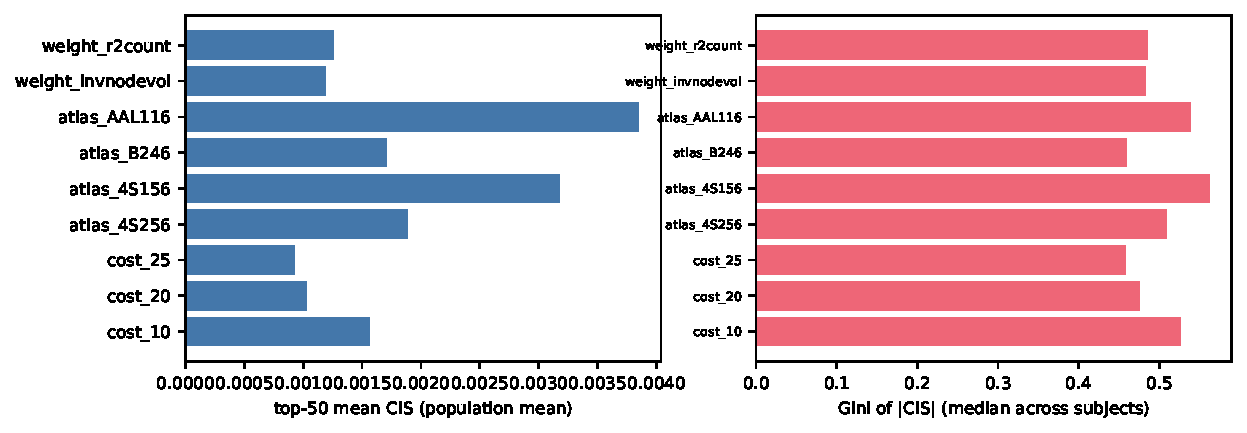
\includegraphics[width=\textwidth]{fig07_robustness.pdf}
\caption{\textbf{Robustness ladder (9 configurations, $n=150$ per
configuration).} Top-50 mean-of-means and Gini across atlases \{4S256,
4S156, Brainnetome246Ext, AAL116\}, weights \{\texttt{sift\_invnodevol},
\texttt{radius2\_count}\}, and costs \{0.10, 0.20, 0.25\}. All 9
configurations reproduce the primary architecture; the maximum like-for-like
top-50-mean deviation is 0.00262 (atlas AAL116; no numeric tolerance was
pre-registered for E06 --- descriptive comparison).}
\label{fig:supprobust}
\end{figure}

\section{Seeds}
Subject samples: one RNG, seed 20260922, nested samples (A $\subset$ B).
Nulls: $100+i$ per graph. Enrichment/rank-stability: 20260922. All recorded
in \path{null_manifest_battery_a.csv} and script constants.

\section{Additional distributions}
Null $\delta/z$ distributions: \path{battery_a/*.npz} (100 $\times$ 456
null-CIS matrices per subject), \path{null_results_battery_b.csv}
(per-subject null mean/sd). Per-subject CIS:
\path{04_CIS/subject_cis/sub-<subjectID>.csv} (456 rows each, 900 files).
Baseline: \path{09_TABLES/table_baseline_network_properties.csv}.
Highest-stability nodes: Table~\ref{tab:stopnodes}.

% Auto-generated float (caption + label inside the file):
% AUTO-GENERATED from 09_TABLES/table_05_top_stability.csv -- do not edit numbers by hand.
\begin{table}[!t]
\centering\small
\caption{Eight highest-ranked nodes by population-mean CIS (frozen
\texttt{table\_05\_top\_stability.csv}): mean CIS across the 801-subject
cohort, mean degree, fraction of subjects in which the node falls in the
top-50 (\texttt{top50\_rate}) and top decile (\texttt{topdecile\_rate}) CIS.
Node indices follow the frozen 4S456 atlas manifest.}
\label{tab:stopnodes}
\begin{tabular}{crrrrr}
\toprule
Rank & Node & mean CIS & mean degree & top-50 rate & top-decile rate \\
\midrule
1 & 415 & 0.0037 & 226.9 & 1.000 & 1.000 \\
2 & 401 & 0.0034 & 213.8 & 1.000 & 1.000 \\
3 & 414 & 0.0046 & 235.9 & 1.000 & 1.000 \\
4 & 400 & 0.0043 & 226.9 & 1.000 & 1.000 \\
5 & 442 & 0.0020 & 159.1 & 0.993 & 0.992 \\
6 & 451 & 0.0020 & 143.5 & 0.987 & 0.979 \\
7 & 444 & 0.0018 & 157.5 & 0.982 & 0.976 \\
8 & 97 & 0.0012 & 160.6 & 0.968 & 0.958 \\
\bottomrule
\end{tabular}
\end{table}


\section{Anatomical mapping}
\path{00_MANIFEST/manifests/atlas_4S456_system_labels.csv} (456 nodes;
Vis 61, SomMot 77, DorsAttn 46, SalVentAttn 47, Limbic 26, Cont 52, Default
91, Subcortical\_Cerebellar 56). Human chokepoint catalogue:
\path{07_CROSS_SCALE/human_chokepoint_catalogue.csv}.

\section{Literature novelty matrix}
\path{10_LITERATURE/NOVELTY_MATRIX.md} (+ Kudriavtsev gate record:
\path{10_LITERATURE/KUDRIAVTSEV_2026_FULLTEXT_REVIEW.md}).

\section{Reproducibility instructions}
\begin{enumerate}
\item \texttt{git clone} the repository (heavy data excluded; raw zips from
Zenodo).
\item Run \path{02_PREPROCESSING/preprocess_v2.py} (rebuilds
\path{cache_parts/}, resume-safe) $\to$
\path{03_BASELINE/baseline.py} $\to$ \path{04_CIS/cis_primary.py}
$\to$ \path{05_NULLS/degree_preserving/null_models.py} \texttt{--battery a|b}
$\to$ \path{04_CIS/e05_statistics.py} $\to$
\path{06_ROBUSTNESS/robustness.py} $\to$
\path{09_TABLES/build_tables.py} $\to$ \path{08_FIGURES/make_figures.py}.
\item Numeric audit without any recomputation:
\texttt{python} \path{10_REPORT/verify_final_numbers.py} (stdlib-only; 46
checks).
\item Environment: Python 3.13, numpy 2.4.2, scipy 1.18.0, pandas 2.3.3
(see \path{ANALYSIS_FREEZE.md} provenance-gap note).
\end{enumerate}

\section{Conceptual schematic}
Two-layer architecture: a dominant connectivity-dependent component plus a
smaller degree-independent residual, arbitrated by matched controls and
degree-preserving nulls. Schematic only; no data are plotted
(Fig.~\ref{fig:schem}).

\begin{figure}[!t]
\centering
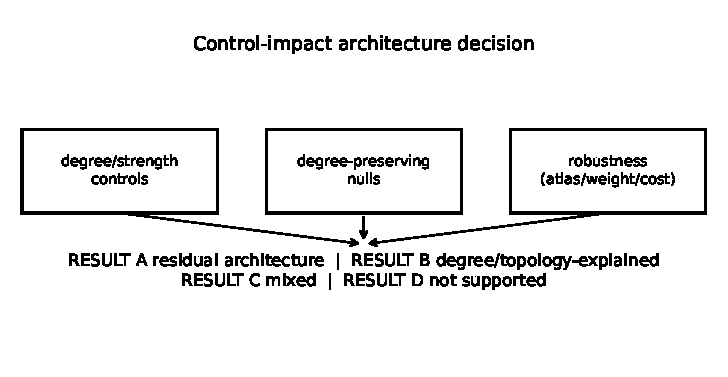
\includegraphics[width=0.72\textwidth]{fig09_conceptual.pdf}
\caption{\textbf{Conceptual schematic.} Two-layer architecture: a dominant
connectivity-dependent component plus a smaller degree-independent residual,
arbitrated by matched controls and degree-preserving nulls. Schematic only;
no data are plotted.}
\label{fig:schem}
\end{figure}

\end{document}
